%!TEX program = xelatex
\documentclass[10pt]{beamer}

\usetheme[progressbar=frametitle]{metropolis}
% \setbeamerwidth{text margin left=0.2in, text margin right=0.2in}

\usepackage{booktabs}
% \usepackage[scale=2]{ccicons}
% \usepackage{FiraSans}
\usepackage{changepage}
\usepackage{caption}

\usepackage{pgfplots}
\usepgfplotslibrary{dateplot}

\newcommand\Wider[2][3em]{%
\makebox[\linewidth][c]{%
  \begin{minipage}{\dimexpr\textwidth+#1\relax}
  \raggedright#2
  \end{minipage}%
  }%
}

\title{Linear Classification Methods and QDA}
\date{February 25, 2016}
\author{John Ensley \& Songshan Yang}
\institute{Penn State University \\ STAT 557}
\titlegraphic{\hfill
\includegraphics[height=1.75cm]{../images/psulogo.png}}

\begin{document}

\metroset{block=fill}

\maketitle

% \begin{frame}
%   \frametitle{Table of Contents}
%   \setbeamertemplate{section in toc}[sections numbered]
%   \tableofcontents[hideallsubsections]
% \end{frame}


\begin{frame}\frametitle{Data Description}
\begin{itemize}
  \item 699 tumor samples
  \item 458 classified as benign, 241 as malignant
  \item 9 observations for each: uniformity of cell size, uniformity of cell shape, marginal adhesion, single epithelial cell size, bare nuclei, bland chromatin, normal nucleoli, mitoses
  \item Each predictor is a value from 1 to 10
\end{itemize}
\end{frame}

\begin{frame}\frametitle{Results, No Dimension Reduction}

50\% of observations randomly chosen for training data, rest used for testing
  \begin{center}
  \begin{tabular}{cccc}
    \toprule
    Method & LDA & QDA & Logistic Regression \\
    \midrule
    Error Rate & 0.0395 & 0.0401 & 0.0307 \\
    \bottomrule
  \end{tabular}
  \end{center}

\end{frame}

\begin{frame}\frametitle{Principal Component Analysis}
  \begin{center}
    \resizebox{\textwidth}{!}{%
    \begin{tabular}{c|ccccccccc}
      \toprule
      PCs & 0.655 & 0.086 & 0.060 & 0.051 & 0.042 & 0.034 & 0.033 & 0.029 & 0.010 \\
      \bottomrule
    \end{tabular}}
    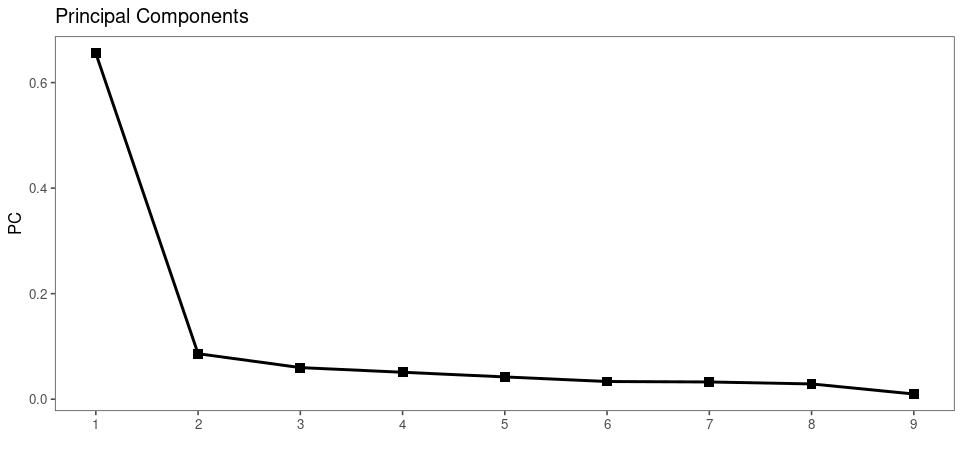
\includegraphics[width=0.9\textwidth]{../images/pca.png}
  \end{center}

  The first 2 principal components make up 74\% of the variance
\end{frame}

\begin{frame}\frametitle{Results, Dimension Reduction}
  50\% of observations randomly chosen for training data, rest used for testing
  \begin{center}
  \begin{tabular}{cccc}
    \toprule
    Error Rates & LDA & QDA & Logistic Regression \\
    \midrule
    Original Data & 0.0395 & 0.0401 & 0.0307 \\
    2 PCs & 0.0395 & 0.0337 & 0.0307 \\
    \bottomrule
  \end{tabular}
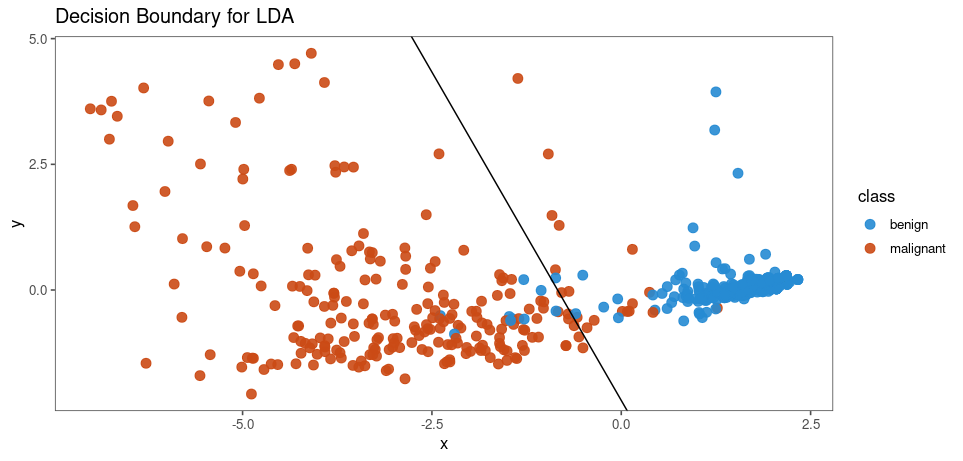
\includegraphics[width=0.9\textwidth]{../images/lda.png}
  \end{center}
\end{frame}

\begin{frame}\frametitle{Results, Cross Validation}
  \begin{center}
  \begin{tabular}{cccc}
    \toprule
    10-fold CV & LDA & QDA & Logistic Regression \\
    \midrule
    Original Data & 0.0395 & 0.0483 & 0.0351 \\
    2 PCs & 0.0395 & 0.0337 & 0.0307 \\
    \bottomrule
  \end{tabular}
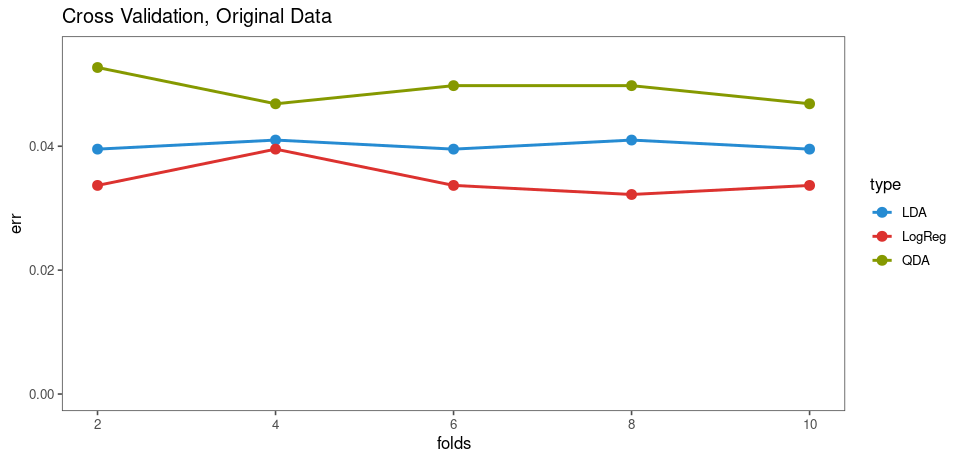
\includegraphics[width=0.6\textwidth]{../images/cv-nopc.png} \\
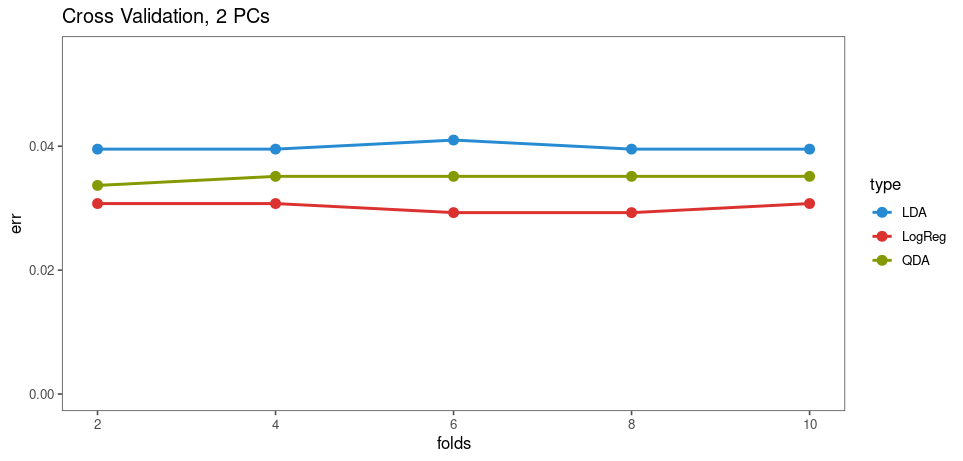
\includegraphics[width=0.6\textwidth]{../images/cv-pc.png}
  \end{center}
\end{frame}

\begin{frame}\frametitle{Results, Cross Validation}
  \begin{center}
    No PCA:
    \begin{tabular}{c|ccc}
      \toprule
      Folds & LDA & QDA & Logistic Regression \\
      \midrule
      2 & 0.0468 & 0.0454 & 0.0410 \\
      4 & 0.0395 & 0.0512 & 0.0322 \\
      6 & 0.0395 & 0.0468 & 0.0307 \\
      8 & 0.0395 & 0.0483 & 0.0307 \\
     10 & 0.0395 & 0.0483 & 0.0351 \\
      \bottomrule
    \end{tabular}

    \vspace{10pt}
    
    PCA:
    \begin{tabular}{c|ccc}
      \toprule
      Folds & LDA & QDA & Logistic Regression \\
      \midrule
      2 & 0.0380 & 0.0351 & 0.0366 \\
      4 & 0.0380 & 0.0337 & 0.0292 \\
      6 & 0.0395 & 0.0351 & 0.0322 \\
      8 & 0.0395 & 0.0351 & 0.0307 \\
     10 & 0.0395 & 0.0337 & 0.0307 \\
      \bottomrule
    \end{tabular}
  \end{center} 
\end{frame}

\begin{frame}\frametitle{Conclusions}
  \begin{itemize}
    \item All classification methods perform well on this dataset
    \item Logistic regression performs the best overall
    \item Using 2 principal components improves the error rates, particularly with QDA
  \end{itemize}
\end{frame}



\end{document}
